
\section{Toy model Comparisons}
To evaluate the introduced greedy approach, its performance was tested on randomly generated toy models. The models contained 12 to 30 particles that were randomly distributed in space. The particles were randomly assigned to two entities, representing two molecules. A selection of four restraints was simulated with no preprocessing filtering steps. Different algorithmic approaches were applied in the simulated selections: the introduced greedy approach, a 100 times repeated random selection, and two brute force approaches were used. One brute force approach maximized the distance between the selected restraints, and the other brute force approach maximized the CHV around the selected restraints like it is done for multistate system chaining. Each number of particles was sampled 20 times to give an insight into the uncertainty estimate of the particle placement. The scripts for this approach can be found in the example folder of our repository.

\subsection{Systems}
The systems for which the relative hydration free energies were calculated are selected sub-sets of the ATB Solvation Free Energy Database \cite{Martin2018}.

The solvation free energy calculations with the pairwise TI were carried out on a subset of $16$ molecules leading to 15 relative hydration free energies. The selected molecules represent transformations such as R-group changes and ring size changes, but also scaffold hopping transformations.

\begin{figure}[h]
    \centering
    
\includegraphics[width=\textwidth]{fig/methods/StateGraph_TI_2D.png}
    \caption{TI-Graph. In order to evaluate the restraints generated by RestraintMaker, a set of 16 molecules was chosen from the ATB Database.\cite{Martin2018} The set was chosen so it contained both relatively similar molecules with identical cores, as well as more difficult transformations such as scaffold hopping. The RestraintMaker was used to generate pairwise distance restraints between molecule M030 and the other molecules of the set. The relative hydration free energies were then calculated using TI with a linked dual topology approach with the generated distance restraints .}
    \label{fig: Pairwise_TI_M030_Graph}
\end{figure}

To apply our approach to multistate systems, two sub-sets of molecules were generated from the set of molecules selected for the pairwise TI simulations. The first subset A contains six molecules with the same core and transformations like R-group changes.

The second subset B for the multistate simulations increases the number of states and consists of 10 molecules. In this set, the complexity of the transformations is increased by a ring size change and a ring flexibility change.

\begin{figure}[h]
    \centering
    \begin{subfigure}{0.40\columnwidth}
        
\includegraphics[width=\textwidth]{fig/methods/StateGraph_Multistate_easy6_2D.png}
        \caption{}
        \label{fig: multistate_6LigandsGraph}
    \end{subfigure}
    \begin{subfigure}{0.55\columnwidth}
        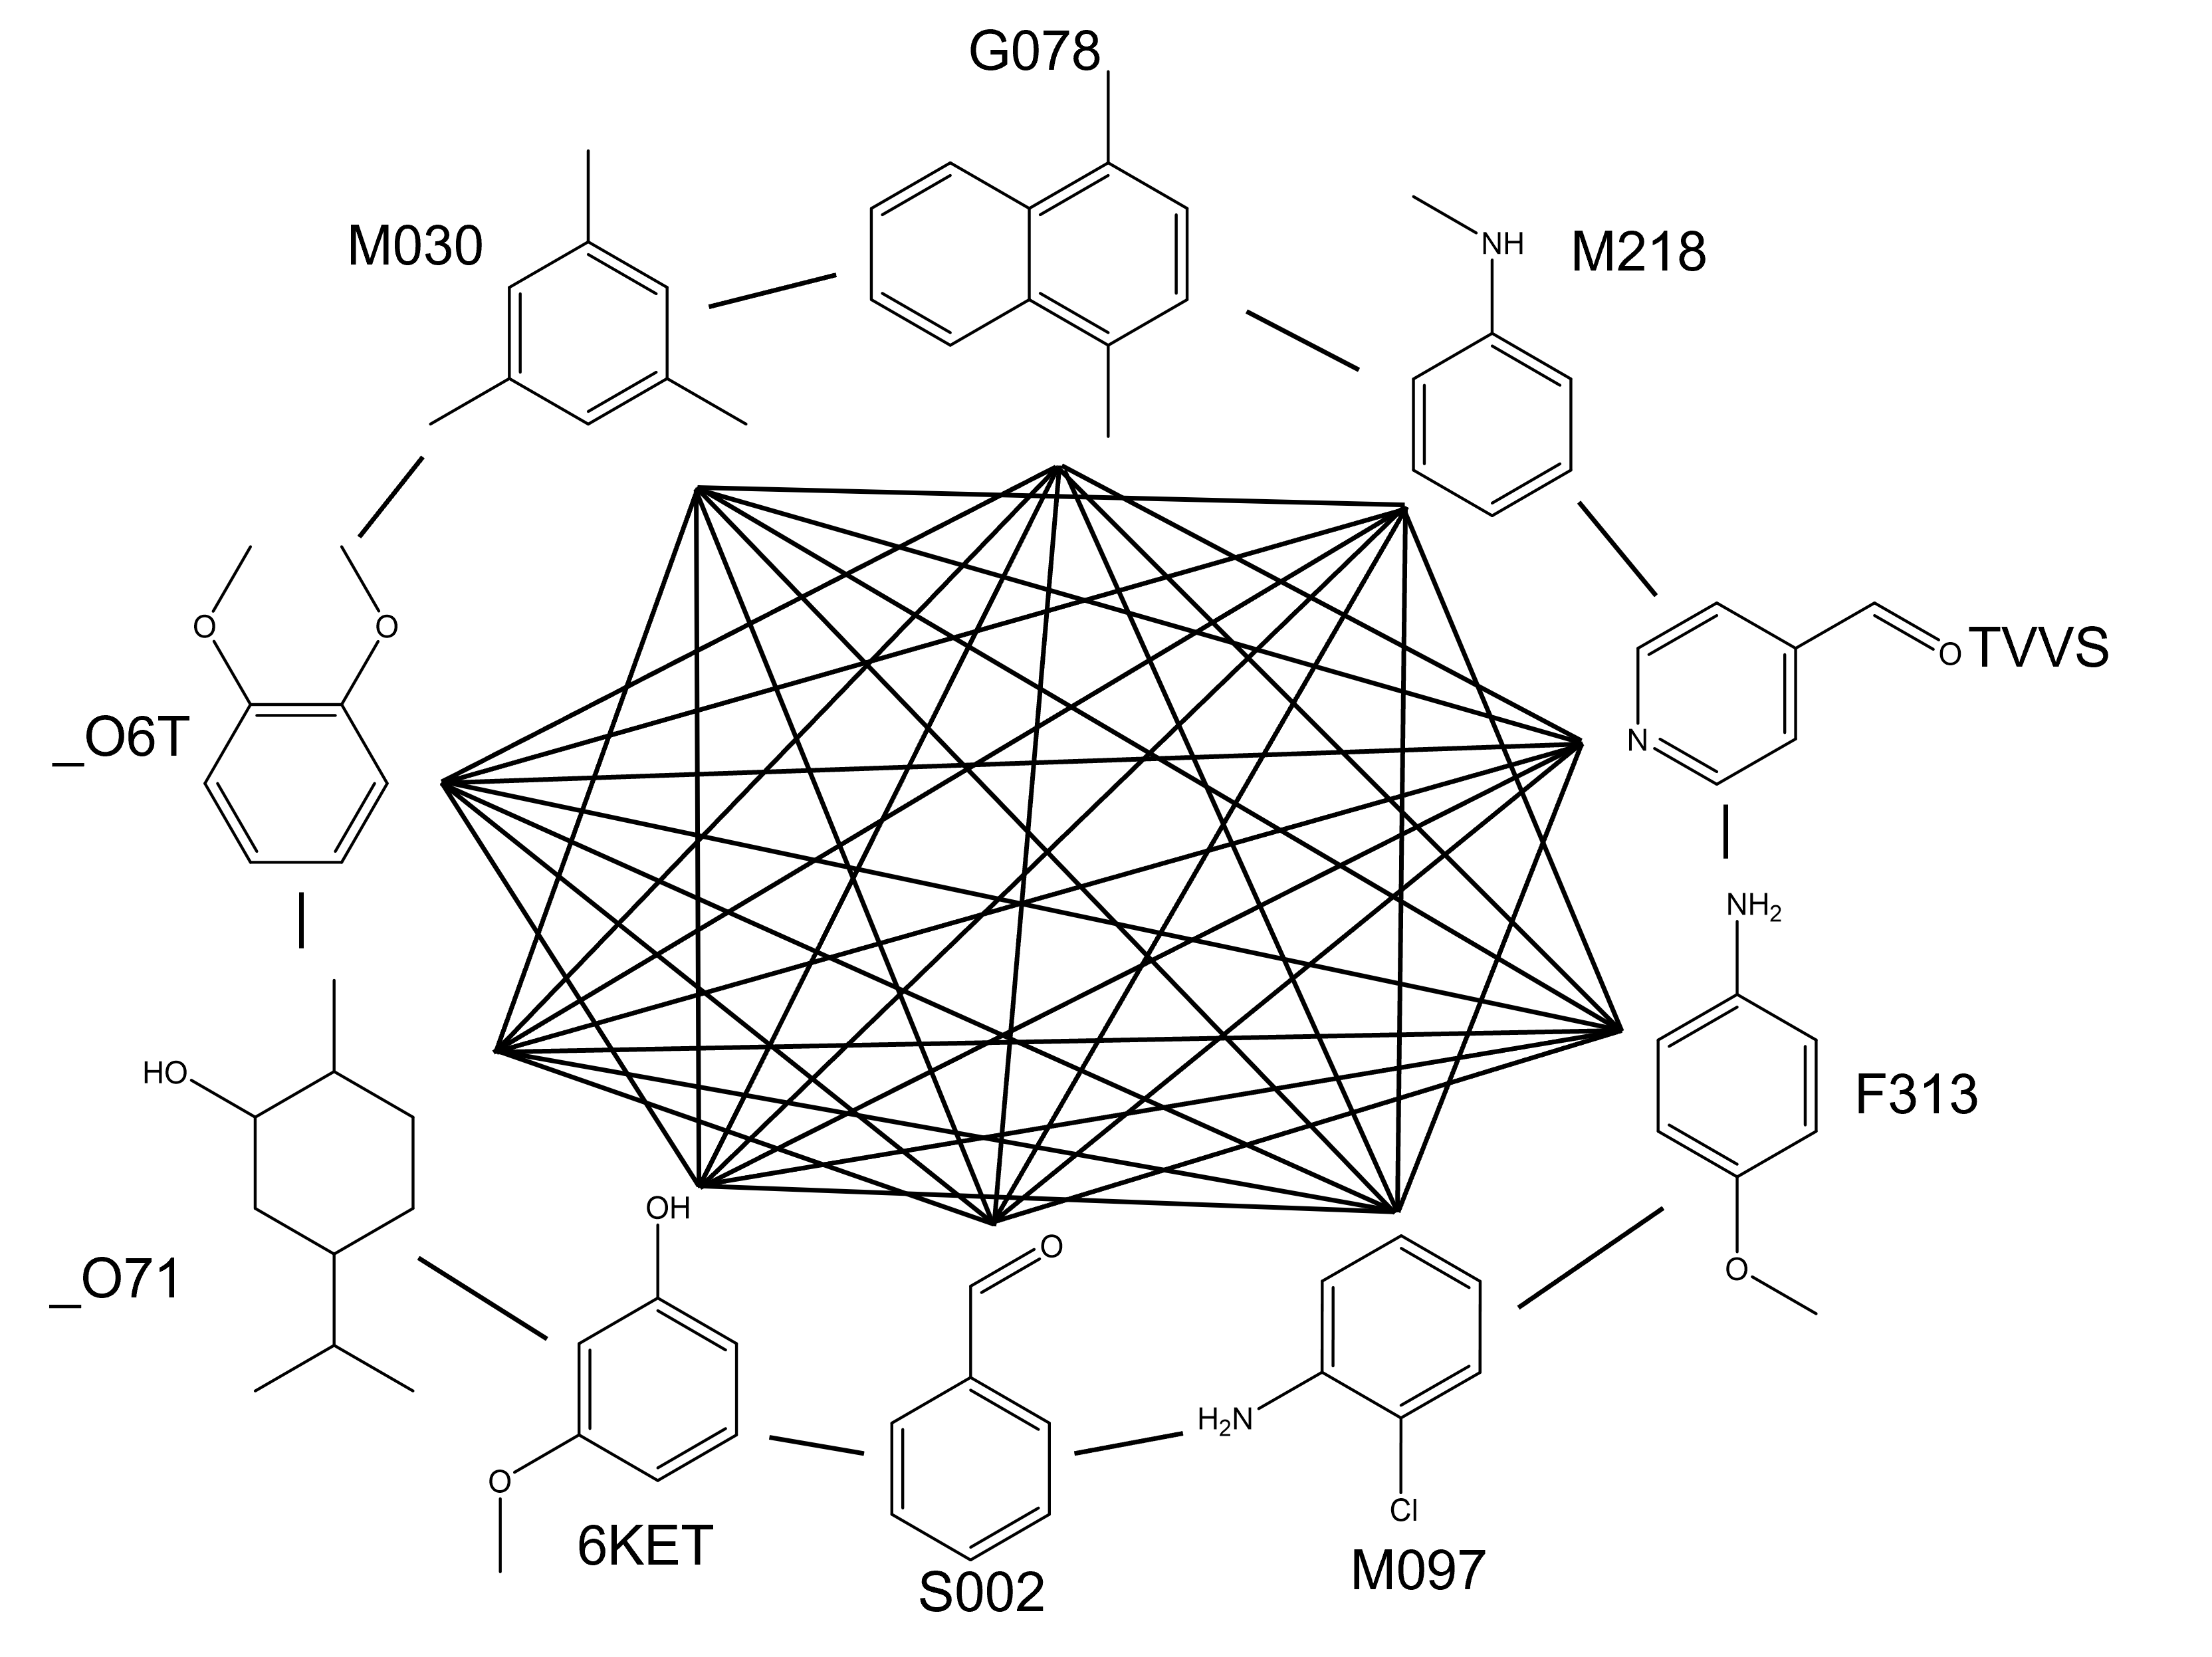
\includegraphics[width=\textwidth]{fig/methods/10state_flat_graph_2D.png}
        \caption{}
        \label{fig: multistate_10LigandsGraph}.
    \end{subfigure}
    \caption{Overview of the multistate systems. Two subsets were formed from the chosen molecules in Fig. \ref{fig: Pairwise_TI_M030_Graph} and all the possible transformation paths are indicated. \ref{fig: multistate_6LigandsGraph} Set A consists of six molecules, that contain mainly R-group and polarity transformations. \ref{fig: multistate_10LigandsGraph} Set B consists of 10 molecules that add to the transformations of set A ring flexibility changes}
    \label{fig: Subsets}
\end{figure}

The sets of molecules are depicted in Figures \ref{fig: Pairwise_TI_M030_Graph}, \ref{fig: multistate_6LigandsGraph}, and \ref{fig: multistate_10LigandsGraph}, respectively.

\subsection{Simulation Details}
The simulations were carried out using the molecular dynamics package GROMOS version 1.5.0 (freely available on \textit{http://www.gromos.net}),
the python RE-EDS pipeline package (\textit{https://github.com/rinikerlab/reeds}) 
and PyGromosTools (\textit{https://github.com/rinikerlab/PyGromosTools}). \cite{Schmid2012, Ries2021, Lehner2021} 

In order to compare the simulated results to the results reported in the ATB database, the same simulation setup was used. The topologies were taken from the ATB database. All simulations in water were carried out using the single-point charge (SPC) water model.\cite{Berendsen1981}. A single cutoff radius of $1.2$~nm was used for the calculation of the non-bonded interactions. The integration time step was set to $2$~fs and the pairlist was updated every five steps. Long-range nonbonded interactions were calculated using a reaction field correction with $\varepsilon_{rf}=1$ for the simulations in vacuum and $\varepsilon_{rf}=61$ for the simulations in water.\cite{tironi1995} The force constant for the distance restraints was set to $5000$ kJ$/($mol$\cdot$nm$)$.

\subsubsection{TI}
The thermodynamic integration was prepared by a short energy minimization with maximally 30000 steps and minimally $2000$ steps, converging if the potential energy is not changing anymore for larger values then $0.1~kJ$ . Next the TI was carried out with $21$ evenly spaced $\lambda$-windows between $1$ and $0$, both for water and vaccum environment. Each window was equilibrated for $1~$ns and afterwards a production run of $5~$ns was carried out. The free energies were calculated using the simpson integration of SciPy.\cite{Virtanen2020}

\subsubsection{RE-EDS}
The topologies for the RE-EDS calculations were prepared using PyGromosTools.\cite{Lehner2021} The simulations were carried out using the RE-EDS pipeline of Ries et al.\cite{Ries2021}.

For set A, six EDS simulations of $2$~ns were carried out in vacuum/water to generate optimized state configurations. 21 EDS simulations with s-values distributed logarithmically between $1$ and $10^{-5}$ were run for $200$~ps to determine the lowest s-value for the RE-EDS simulations such that undersampling was observed. For the simulations in vacuum, the lowest s-value was determined to be $0.00316$. For the simulations in water, the lowest s-value was determined to be 0.001. Next, the energy offsets were estimated from $800$~ps RE-EDS simulations. For the vacuum simulations, $12$ replicas were used and for the water simulations, $14$ replicas were used. In vacuum, one s-optimization run of $500$~ps was enough to ensure that roundtrips occurred in all replicas and all states were sampled well. 4 replicas were added. In water, three s-optimization runs of $500$~ps, $1000$~ps and $1500$~ps, respectively, were used to achieve roundtrips in all replicas. After each s-optimization run, five replicas were added. Additionally, for the simulation in water, the energy offsets were rebalanced during three $500$~ps RE-EDS energy offset rebalancing runs to ensure that all states were sampled equally. This was not necessary for the vacuum simulations, as all states were already sampled well after the s-optimization. Finally, a $500$~ps RE-EDS simulation was used to calculate the free energy differences in vacuum. In water, a $1$~ns RE-EDS simulation was used to calculate the free energy differences.

For set B, ten EDS simulations of $2$~ns were used in vacuum/water to generate optimized configurations for the ten molecules. As for set A, $21$ $200$~ps EDS simulations were carried out with logarithmically distributed s-values between $1$ and $10^{-5}$. The lowest s-value for the vacuum simulations was determined to be $0.00178$, and for the simulations in water $0.001$. For the energy offset estimation a $800$~ps RE-EDS simulation was used. For the simulation in water, $18$ replicas were used and for the simulation in vacuum, $17$ replicas were used. As for set A, only one s-optimization RE-EDS simulation of $500$~ps was needed in vacuum. Again, $4$ replicas were added. However, for the simulation in water, five s-optimzation runs of $500$~ps, $1000$~ps, $1500$~ps, $1500$~ps and $1500$~ps, respectively, were needed to ensure sufficient roundtrips in all replicas. At each s-optimization iteration, five replicas were added. While the energy offset rebalancing step could again be skipped for the simulation in vacuum, the energy offsets for the water simulation were rebalanced in 5 RE-EDS runs of $500$~ps. In order to determine the free energy differences in vacuum, a $1$~ns RE-EDS simulation was carried out. A $5$~ns RE-EDS production run was used to calculate the free energy differences in water.

More details on the RE-EDS pipeline and its substeps can be found in the work of Ries et al.\cite{Ries2021}

\subsection{Analysis}
The analysis of the simulations was done using \textit{GROMOS++} \cite{eichenberger2011} and PyGromosTools \cite{Lehner2021}. Further, the  following python packages were used for the statistical analysis and plotting: pandas \cite{Mckinney2010}, Matplotlib \cite{Hunter2007}, NumPy \cite{VanDerWalt2011}, SciPy \cite{Virtanen2020}, mpmath \cite{Johansson2013} and Jupyter notebooks.\cite{Kluyver2016}.